\chapter{\eloismeretek}

\section{Esettanulmány}
A dolgozatban elért eredményeket a Train Benchmark \cite{szarnyas2018train} esettanulmány segítségével fogom bemutatni. Ez a benchmark azért jött létre, hogy összetudjuk hasonlítani különböző gráflekérdező rendszerek teljesítményét főleg időigény és memória felhasználás szempontjából. Ehhez többek között definiálja a vasút rendszer metamodelljét. Munkám során ezt a metamodellt felhasználva generáltam lekérdezéseimet, ezért bemutatom, hogy milyen elemekből áll. 

\begin{figure}
	\centering
	\includegraphics[width=0.7\textwidth]{figures/trainbenchmarkfig1}
	\caption{Vasúti útvonal részlet (forrás: \cite{szarnyas2018train})}
	\label{fig:trainbenchmark}
\end{figure}

 \Aref{fig:trainbenchmark}-es ábrán látható egy a trainbenchmark metamodelljére alapuló részlet. Ebben a kontextusban egy vasúti útvonal nem más mint szegmensek és váltók sorozata, illetve a belépést és a kilépést egy-egy szemafor jelzi. Ahhoz hogy biztonságos legyen a közlekedés szükség van szenzorokra, amelyek monitorozzák a különböző szegmensek és váltók kihasználtságát. Egy útvonal definiálásához ,a felsorolt elemeken kívül a váltók adott útvonalhoz tartozó pozícióját is el kell tárolnunk. Egy útvonal akkor aktív, ha a rendszerben a specifikációjának megfelelően állnak a váltók.

A metamodellezés egy tecknika arra, hogy definiájunk modellező nyelveket, ahol a metamodell specifikálja a nyelv szintaktikáját. A trainbenchmark metamodellje \aref{fig:trainbenchmarkmetamodell} -es ábrán látható.

\begin{figure}
	\centering
	\includegraphics[width=0.7\textwidth]{figures/trainbenchmarkfig2}
	\caption{A train benchmark metamodellje. a, tartalmazási hierarchia és relációk b, öröklési relációk (forrás: \cite{szarnyas2018train})}
	\label{fig:trainbenchmarkmetamodell}
\end{figure}


\section{Gráflekérdező rendszerek}
A gráfok intuitív formalizációt nyújtanak modellezési szempontból arra, hogy úgy írhassuk le a világot ahogy az ember gondolkozik róla. Tehát mint dolgok (csomópontok) és köztük lévő kapcsolatok (élek) \cite{marton2017model}. A property gráf adatmodell kiterjeszti a gráfokat úgy, hogy címkéket/típusokat illetve tulajdonságokat ad a csúcsoknak és az éleknek. A gráf adatbázisok  alkalmasak tulajdonság gráfok tárolására, és az abban lévő adatok lekérdezésére komplex gráf minták használatával. Ilyen rendszerek például a    Neo4j \cite{neo4j}, OrientDB \cite{orientdb} és a  SparkSee \cite{sparksee}.

\begin{figure}
	\centering
	\includegraphics[width=0.7\textwidth]{figures/tulajdonsággráfpélda}
	\caption{Property gráf példa(forrás: \cite{marton2017model})}
	\label{fig:tulajdonsággráfpélda}
\end{figure}

Ahhoz hogy jobban megérthessük mi is ez az adatmodell \aref{fig:tulajdonsággráfpélda} -es ábrán látható egy példa.
\subsection{Neo4j}

A Neo4J egy populáris NoSQL property gráf adatbázis és a Cypher lekérdező nyelvet kínálja lekérdezések írására. A Cypher egy magas szintű deklaratív lekérdező nyelv és mivel le van választava a lekérdező rendszerről, ezért az képes a Cypher nyelven írt lekérdezések optimalizálására. 
A Cypher szintaxisa olyan gráf minták megírását teszi lehetővé, amelyeknek megértése nagyon egyszerű. \Aref{fig:példalekérdezes} -es példán egy olyan lekérdezést láthatunk,  ami az összes olyan vonat, szegmens párral tér vissza, ahol az adott vonat rajta van az adott szegmensen.  

\begin{figure}
	\begin{lstlisting}[style=viatrasmall]
	MATCH (tr:Train)-[:ON]->(seg:Segment)
	RETURN tr, seg	
	\end{lstlisting}   
	\caption{Példalekérdezés(forrás: \cite{marton2017model} )}
	\label{fig:példalekérdezes}
\end{figure}


\section{Modellezés és metamodellezés}
A metamodellek definiálják a legfontosabb fogalmakat, relációkat és attribútumokat a cél domainen , hogy 
specifikálják modellek alap struktúráját \cite{semerath2017formal}. Dolgozatomban az Eclipse Modeling Framework
 (EMF) \cite{EMF} -öt használtam metamodellezésre.



\subsection{Cypher query-k metamodellje}
\Aref{fig:cyphermetamodell} -ös ábrán látható a korábban említett Cypher nyelv egyszerűsített metamodellje. A \mm{SinglePartQuery} elem reprezentálja a modell gyökerét. Egy ilyen elem két részből áll : Egy \mm{Match} és egy \mm{Return} elemből. A \mm{Match} elem minták összességéből áll (\mm{Pattern}), amelyek részekre (\mm{PatternPart}) bonthatóak. Egy ilyen részben pedig vagy tartalmaz változó deklarációt, vagy egy belső részt tartalmaz ami taltalmaz változó deklarációt. (\mm{Variable Declaration}). Ezáltal az összes változót a \mm{Match} elemen belül deklaráljuk. A \mm{Return} elem  pedig egy kifejezést (\mm{Expression}) tartalmaz, amelyben mindenképp szerepel egy változó referencia (\mm{VariableRef}) is, így összekötve egymással a \mm{Match} és a \mm{Return} elemet. 

\begin{figure}
	\centering
	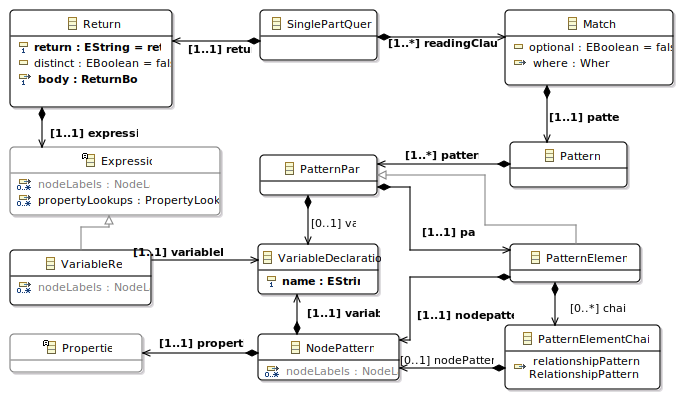
\includegraphics[width=0.7\textwidth]{figures/openCypherClassDiagram}
	\caption{Cypher metamodell}
	\label{fig:cyphermetamodell}
\end{figure}


\subsection{xText}
Az Xtext keretrendszer programozási nyelvek  és  domain-specifikus nyelvek fejlesztésére készül. Az Xtext  
egy erős nyelvtani szabályokkal rendelkező nyelvet használ az egyéedi nyelvtanok definiálására. Ezáltal
egyszerre biztosít parszolót, linkelőt, helyesírásellenőrzőt és fordítót. És a felhasználó hatázohatja 
meg a nyelvének célformátumát is.Ahhoz, hogy a Cypher nyelven megírt lekérdezéseket értelmezni lehessen 
\aref{fig:cyphermetamodell}-ös metamodellen megismert elemek szintjén egy XText \cite{xText} keretrendszerben
íródott nyelvtanra van szükség. A dolgozatomban a slizaa\cite{slizaa_2018} által készített nyelvtanra építettem.


\subsection{\textsc{Viatra} jólformáltsági kényszerek}

\section{Gráfgenerálás}

ábra milyen bemenetek milyen kimenetek





